\documentclass[11pt]{article}

\usepackage{mtsxiv}
%\usepackage{url}
\usepackage[colorlinks=true,citecolor=black,linkcolor=black,urlcolor=blue]{hyperref}
%\usepackage{times}
\usepackage{multirow}
\setlength\titlebox{6.5cm}    % Expanding the titlebox



\usepackage{polyglossia}
\setdefaultlanguage[variant=australian]{english}
\usepackage{latexsym}
\usepackage[small,bf]{caption}
\usepackage{xltxtra}

\usepackage{fontspec}
\defaultfontfeatures{PunctuationSpace=3,Scale=MatchLowercase,Mapping=tex-text}
\newfontfeature{IPA}{+mgrk}
%\setromanfont[IPA]{FreeSerif}
\setromanfont[Scale=0.9]{Times New Roman}
\newfontfamily\qipa[IPA,Scale=MatchLowercase]{FreeSerif}
\setmonofont[Scale=0.7]{DejaVu Sans Mono}

\newcommand{\email}[1]{\texttt{\href{mailto:#1}{#1}}}
\usepackage{natbib}
%\usepackage{natbib,natbibspacing}
\usepackage{setspace}
\usepackage{booktabs}


%\usepackage{subfigure}
%\usepackage{subfloat}
\usepackage{subfig}

%\setlength{\bibspacing}{\baselineskip-0.4em}

\newenvironment{itemise}[1]{
        \begin{itemize}\setlength{\itemsep}{-0.3em}
		  %\setlength{\itemindent}{-1em}
		  %\setlength{\leftmargin}{-2em}
        \vspace{-0.6em}
        #1
}{
        \end{itemize}
        \vspace{-1pt}
}


%\setlength\titlebox{6.5cm}    % You can expand the title box if you
% really have to

\newcommand{\tag}[1]{{\small{\texttt{#1}}}}

%%\Keywords{Kazakh, Tatar, MT, Free software, Open-source}

\newcommand{\confname}{Machine Translation Summit XIV}
\newcommand{\website}{\protect\url{http://www.mtsummit2013.info/}}
\newcommand{\contactname}{research track co-chair Mikel L.\ Forcada}
\newcommand{\contactemail}{mlf@dlsi.ua.es} 
\newcommand{\conffilename}{mtsxiv}
\newcommand{\downloadsite}{\protect\url{http://www.mtsummit2013.info/}}
\newcommand{\paperlength}{$8$ (eight)}
\newcommand{\shortpaperlength}{$4$ (four)}

\title{A free/open-source Kazakh-Tatar machine translation system}

\author{Ilnar Salimzyanov\\
  Kazan Federal University\\
  Kazan, Republic of Tatarstan\\
  Russian Federation\\
  \email{ilnar.salimzyan@gmail.com}  \And
  Jonathan North Washington\\
  Departments of Linguistics\\
  and Central Eurasian Studies\\
  Indiana University\\
  Bloomington, Indiana 47405 USA\\
  \email{jonwashi@indiana.edu}  \And
  Francis Morton Tyers\\
  Departament de Llenguatges\\
  i Sistemes Informàtics\\
  Universitat d'Alacant\\
  E-03877 Alacant\\
  \email{ftyers@dlsi.ua.es}}

\date{\today}






\begin{document}
\spacing{1}
\maketitle
\begin{abstract}
This paper presents a bidirectional machine translation system between Kazakh and Tatar.
\end{abstract}
%FIXME
%\maketitleabstract

\section{Introduction}

This paper presents a prototype shallow-transfer rule-based machine translation
system between Kazakh and Tatar.

The paper will be laid out as follows: Section~\ref{sec:lang}\ gives a brief
description of the two languages; Section~\ref{sec:prev}\ gives a short review
of some previous work in the area of Turkic--Turkic language translation;
Section~\ref{sec:sys}\ describes the system and the tools used to construct it;
Section~\ref{sec:eval}\ gives a preliminary evaluation of the system; and
finally Section~\ref{sec:conc}\ describes our aims for future work and some
concluding remarks.

\section{Previous work}
\label{sec:prev}

Within the Apertium project, work on MT systems between Turkic languages has been started (Turkish-Kyrgyz, Azeri-Turkish), but the Kazakh-Tatar system described by the present study is the closest to production-ready of them.  Among these systems is a prototype Tatar-Bashkir machine translation system which was built by the authors of this paper \citep{tyerswashingtonsalimzyanbattalov12}; due to the closeness of these languages, it proved to provide high accuracy in its translations, but being a prototype system by design, had relatively low coverage.

Besides these systems, several previous works on making machine translation systems between Turkic languages exist, although to our knowledge none are publically available.
Some MT systems have been reported that translate between Turkish and other Turkic languages, including Turkish-Crimean Tatar \citep{altintas01},
Turkish-Azerbaijani \citep{hamzaoglu93}, Turkish-Tatar \citep{suleymanov08}, and
Turkish-Turkmen \citep{tantug07}, though none of these have been released to a public audience.

%FIXME: mention tr-az, tr-ky?

%maybe this should be moved to 'Future plans'
Within the Apertium project, work on several Turkic-language MT systems has been started, with the ultimate goal of creating independent but compatible
finite-state transducers for each language.
%% The idea is that we started Kazakh-Tatar pair to be able to take into account
%% characteristics of two more distant Turkic languages, avoiding narrowing
%% ourselves to mutually intellegible Tatar and Bashkir, but generate
%% transducers which are still compatible and very coherent. Bashkir part of the
%% pair will be updated to the latest developments of Tatar transducer, which
%% took place while working on Kazakh-Tatar.

\section{Languages}
\label{sec:lang}

Both Tatar and Kazakh belong to the Kypchak (or Northwestern) group of Turkic
languages.  The spoken and written languages share some level of mutual intelligibility to naïve native speakers, though this is somewhat limited, and is obscured by different orthographical conventions and some opaque correspondences.

Kazakh is primarily spoken in Kazakhstan, where it is the national
language, sharing official status with Russian as an official language.
Large groups of native speakers also exist in China, neigbouring
Central-Eurasian republics, and Mongolia. The total number of speakers is at least 10 million people.

Tatar is spoken in and around Tatarstan by
approximately 6 million people. It is co-official with Russian in Tatarstan ---
a republic within Russia.  A majority of native speakers of both languages are bilingual in Russian. %, and the standard varieties our system FIXMEs are written in Cyrillic.

%FIXME: Contrastive grammar
\subsection{Phonological differences}
%a generalised summary, 2 or 3 small specific examples
As closely related languages, Kazakh and Tatar share many phonological processes, including front-back vowel harmony systems, consonant voicing assimilation, and even a typologically rare consonantal nasal harmony system.  However, the differing details of these processes and the existence of processes unique to each language render Kazakh and Tatar fairly different.  For example, Kazakh has a ubiquitous system of desonorisation of the initial sonorants found in many common morphemes.  Furthermore, Tatar has nasal assimilation of the initial /l/ of the plural-suffix.

\subsection{Orthographic differences}
%a generalised summary, 1 or 2 small specific examples
The standard varieties of Kazakh and Tatar our system deals with are both written in Cyrillic, though their implementations of Cyrillic differ in many ways.

While Tatar and Kazakh both have a velar/uvular obstruent distinction (e.g., /k/ vs.\ /q/) that interacts with adjacent vowels, the Tatar orthography only has one series of letters (e.g., ‹к›), relying on adjacent vowels (and employing ``hard'' and ``soft signs'' when these fail) to differentiate the two, and Kazakh has two series of obstruents (e.g., ‹к› and ‹қ›).

Kazakh does not orthographically distinguish high unrounded vowels (/{\qipa ɘ}/ ‹і› and /ə/ ‹ы›) before glides (/w/ ‹у› and /j/ ‹й›) by writing the combination with one letter; i.e., /{\qipa ɘ}j/ and /əj/ are both written ‹и›, while /{\qipa ɘ}w/ and /əw/ are both written ‹у›.  The quality of these vowels is necessary to know in order to predict the quality of following harmonising vowels. %, so this convention presents accute challenges to producing an accurate morphological transducer.
Additionally, Tatar and Kazakh both use ``yoticised'' vowels---i.e., when ‹о›, ‹у›, or ‹а› (along with ‹ә› in Tatar) follow /j/, a single character is used to represent both: ‹ё›, ‹ю›, and ‹я› respectively.\footnote{Furthermore, in Tatar, /j/ followed by ‹э› or ‹ы› in Tatar is represented by ‹е›, though ‹е› is also the non-word-initial variant of ‹э›.}  %Combined with the issues regarding ‹у› in Kazakh,

All of these orthographical conventions present accute challenges to designing accurate morphological transducers for the languages.

\subsection{Morphological differences}
There are a number of examples where the morphologies of Kazakh and Tatar are rather different, including morphemes in one language that don't exist in the other, entirely different uses of the same morpheme combinations, and morphotactic differences (i.e., allowable ordering and placement of morphemes).

An example of a morpheme that doesn't exist in one of the two languages is Kazakh -\texttt{\{E\}т\{I\}н}, which is used to form non-past verbal adjectives and verbal nouns.  The semantically equivalent structure in Tatar is -\texttt{\{E\} торган}, which historically corresponds to the source of the Kazakh morpheme; however, the use of -\texttt{\{E\} тұрған} in modern Kazakh is different from that of -\texttt{\{E\}т\{I\}н}.

%Another example of a far-reading morphological difference between Tatar and Kazakh reflects the presence of a four-way distinction in Kazakh's 2nd person system, where Tatar only has a two-way distinction.  Kazakh has a distinct pronoun for all combinations of [±plural, ±formal] (сен, сендер, сіз, сіздер), whereas Tatar collapse all pronouns except the [-plural, -formal] син into one pronoun (сез).  This does not only affect affect the pronoun system: since all finite verb forms morphologically agree in person and number with their subject and all possessed nouns agree in person and number with their possessor (with pronouns used in both circumstances only for emphasis and clarification, as is typical in pro-drop languages), the Kazakh and Tatar systems of agreement suffixes have the same pattern.
Another example of a far-reading morphological difference between Tatar and Kazakh reflects the presence of a four-way distinction in Kazakh's 2nd person system, where Tatar only has a two-way distinction.  Kazakh has a distinct pronoun for all combinations of [±plural, ±formal], whereas Tatar collapses all pronouns except the [-plural, -formal] into one pronoun, as summarised in table~\ref{tab:2pprons}  
\begin{table}[htbp]
%\begin{subtables}
	%\begin{subtable}[l]
	%\subtable[Kazakh 2nd person pronouns]{
	%\begin{subtable}
	\subfloat[Kazakh 2nd person pronouns]{
		\begin{tabular}{lll}
			\toprule
			 & -pl & +pl \\\midrule
			-formal & сен & сендер \\
			+formal & сіз & сіздер \\\bottomrule
		\end{tabular}
	%	\caption{Kazakh 2nd person pronouns}
	%\end{subtable}
	%\end{subtable}
	%\begin{subtable}
	%\begin{subtable}
	%}\subtable[Tatar 2nd person pronouns]{
	}\vspace{1.5ex}
	\subfloat[Tatar 2nd person pronouns]{
		\begin{tabular}{lll}
			\toprule
			 & -pl & +pl \\\midrule
			-formal & син & сез \\
			+formal & сез & сез \\\bottomrule
		\end{tabular}%}
	%	\caption{Kazakh 2nd person pronouns}
	%\end{subtable}
	%\end{subtable}
	}
	\caption{The 2nd person pronoun systems of Kazakh and Tatar}
	\label{tab:2pprons}
\end{table}
%\end{subtables}
This systematic difference would seem to be a minor issue, since, as is typical in pro-drop languages, pronouns are only used for emphasis and clarification.  However, this difference between Tatar and Kazakh in the second person system runs much deeper than just the pronoun system.  Since all finite verb forms morphologically agree in person and number with their subject and all possessed nouns agree in person and number with their possessor (even when there is no overt pronoun), the Kazakh and Tatar systems of agreement suffixes reflect the same pattern; i.e., there are several sets of agreement morphemes which have a one-to-one correspondence with the pronouns in each language.

The past tense systems of Kazakh and Tatar have a many-to-many correspondence.  At a basic level, Kazakh differentiates [±eyewitness]\footnote{``Eyewitness'' is a convenient term for this feature, though it may be better expressed as simply ``reliability of knowledge'' (which indeed often equates to whether the knowledge was acquired first-hand or not) in many cases.} (where [-eyewitness] is used for cases of both potentially unreliable information and newly discovered information) and [±recent] in the past tense, whereas Tatar has only three categories: eyewitness, non-eyewitness, and newly-acquired-information---all with no [±recent] distinction.  As an example of the many-to-many correspondence that this results in, Tatar has a single non-eyewitness past tense morpheme (\texttt{-GAн}) while Kazakh has a recent non-eyewitness past (\texttt{-IптI}) and a distant non-eyewitness past (\texttt{-GAн екен-}).  On the other hand, these two non-eyewitness past forms in Kazakh are used for both potentially unreliable information and newly acquired information, whereas in Tatar, non-eyewitness (\texttt{-GAн-}) and newly-acquired-information (\texttt{-GAн- икән}) past forms are distinguished.

Morphotactics of -GAн екен/икән

%\subsection{Morphotactic differences}
%2 or 3 specific examples
%
%%FIXME: Ilnar, I can't think of anything for this...
%% The greetings in Tatar kept a probably older variant of /personal copula ending - question
%% partice/ sequence (Исәнмесез vs Сәлеметсіз бе?), but this doesn't seem to be a good example,
%% as it is very "special case".
%% Although, the possessive endings system is somewhat different, maybe there is something.

%\subsection{Lexical and morphological differences}
%2 or 3 specific examples
%> present progressive
%> ... ?
%
%%FIXME: Ilnar, could you come up with some good examples of this?
%% * no instrumental case in Tatar
%% * only one formal 2p pronoun in Tatar (i.e. Сез) as opposed to Kazakh "Сіз" and "Сіздер"
%% * барыпты - барган (икән), сөйлескелі келдім - сөйләшергә килдем, баратын - бара торган

\subsection{Syntactic differences}

%2 or 3 specific examples
% * Different case governance of postpositions (grep for WARNINGs in bidix)
% * музейлік экспозиция > музей экспозициясе; экспозициялық зал > экспозиция залы
% ** This works, there is a rule for that: if an /adjective + noun/ is translated with /n.attr + noun/, <px3sp> affix is added in Tatar 
% * Мен оқуды жақсы көремін > Мин укырга яратам.
% Also, see this page: http://wiki.apertium.org/wiki/Kazakh_and_Tatar/Pending_tests
There are a number of syntactic differences in Tatar and Kazakh, which include differences in verb valencies in equivalent translations, FIXME, and FIXME.

%FIXME: Ilnar, please check the Tatar
% There is "ошый" in Tatar, which works the same way as Kazakh verb.
% But I found the following in the bidix:

% <e>       <p><l>иемден<s n="v"/><s n="tv"/></l>   <r>ия<b/>бул<s n="v"/><s n="iv"/></r></p></e> <!--"" WARNING transitivity-->
% <e>       <p><l>сақтандыр<s n="v"/><s n="iv"/></l><r>кисәт<s n="v"/><s n="tv"/></r></p></e> <!--"" WARNING: IV<>TV-->
% <e>       <p><l>тұтын<s n="v"/><s n="tv"/></l>    <r>тотын<s n="v"/><s n="iv"/></r></p></e> <!--"" WARNING transitivity-->
% <e>       <p><l>тұтын<s n="v"/><s n="tv"/></l>    <r>тотын<s n="v"/><s n="iv"/></r></p></e> <!--"" WARNING transitivity-->

% There are few other WARNINGs as well.

%FIXME: use a noun in examples, not infinitive/gerund
An example of a difference in verb valencies is with the expression corresponding to ``to like something'' in Kazakh and Tatar.  In Kazakh, the verb ‹ұна› is used, e.g. ‹оқу маған ұнайды› ``I like studying'', where the subject ``I'' in English is expressed through a dative experiencer in Kazakh and the object ``study'' in English is the grammatical subject in Kazakh.  Tatar, on the other hand, uses a verb whose arguments correspond to the arguments of ``to like'' in English, e.g. ‹мин укуны яратам› ``I like studying'', where the first person pronoun is the grammatical subject and ``studying'' is the grammatical direct object.
%(does this count as syntactic?)

> Tatar infinitive (Kazakh ger+nom/acc/dat, Kazakh -GAlI vadv)

\section{System}
\label{sec:sys}

\begin{figure*}[htbp]
\begin{center}
 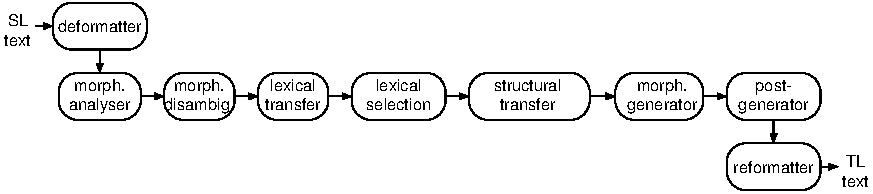
\includegraphics[width=0.8\textwidth]{architecture.pdf}
\end{center}
\caption{The pipeline architecture of the Apertium system.}
\label{fig:modules}
%\vspace{-1em}
\end{figure*}

The system is based on the Apertium machine translation 
platform \citep{apertium/2011}.\footnote{\url{http://www.apertium.org}} The 
platform was originally aimed at the Romance languages of the Iberian peninsula, but has also been adapted for 
other, more distantly related, language pairs.
The whole platform, both programs and data, are licensed under the Free Software Foundation's General Public 
Licence\footnote{\url{http://www.fsf.org/licensing/licenses/gpl.html}} (GPL) and all the software and data for the 
30 supported language pairs (and the other pairs being worked on) is available for download from the project 
website.

\subsection{Architecture of the system}

The Apertium translation engine consists of a Unix-style \emph{pipeline} or
\emph{assembly line} with the following modules (see Fig.~\ref{fig:modules}):  
\begin{itemise}
\item A \emph{deformatter} which encapsulates the format information
 in the input as \emph{superblanks} that will then be seen
 as blanks between words by the other modules.
\item A \emph{morphological analyser} which segments the text in
  surface forms (SF) (\emph{words}, or, where detected, multi-word lexical
  units or MWLUs) and for each, delivers one or more \emph{lexical
    forms} (LF) consisting of \emph{lemma}, \emph{lexical category} and
  morphological information. 
\item A \emph{morphological disambiguator} (constraint grammar) which chooses, using linguistic rules
  the most adequate sequence of morphological analyses for an ambiguous sentence. 
\item A \emph{lexical transfer} module which reads each SL LF 
  and delivers the corresponding target-language (TL) LF
  by looking it up in a bilingual dictionary encoded as an FST
  compiled from the corresponding XML file. The lexical transfer module may
  return more than one TL LF for a single SL LF.
\item A \emph{lexical selection} module which chooses, based on context 
  rules the most adequate translation of ambiguous source language LFs.
\item A \emph{structural transfer} module which
    performs local syntactic operations, is compiled from XML files containing rules that 
    associate an \emph{action} to each defined LF \emph{pattern}. Patterns are applied left-to-right, and the 
    longest matching pattern is always selected.
\item A \emph{morphological generator} which delivers a TL SF
 for each TL LF, by suitably inflecting it. 
\item A \emph{reformatter} which de-encapsulates any format
  information.
\end{itemise}


\subsection{Morphological transducers}

The morphological transducers are based on the Helsinki Finite State Toolkit \citep{hfst/2011}, a free/open-source reimplementation of the Xerox finite-state toolchain, popular in the field of morphological analysis. It implements both the \textbf{lexc} formalism for defining lexicons, and the \textbf{twol} and \textbf{xfst} formalisms for modeling morphophonological rules. It also supports other finite state transducer formalisms such as \textbf{sfst}. This toolkit has been chosen as it --- or the equivalent XFST --- has been widely used for other Turkic languages \citep{coltekin2010,altintas2001,tantug2006,washingtonipasovtyers12,tyerswashingtonsalimzyanbattalov12}, and is available under a free/open-source licence.

The morphologies of both languages are implemented in lexc, and the morphophonologies of both languages are implemented in twol.

Use of lexc allows for straightforward definition of different word classes and subclasses.  For example, Tatar (but not Kazakh) has two classes of verbs: one which takes a harmonised high vowel in the infinitive (the default), and one which take a harmonised low vowel in the infinitive.  This was implemented in lexc with two similar continuation lexica for verbs: one pointing at a lexicon with an A-initial infinitive ending, and another pointing at a lexicon with an I-initial infinitive ending.

Use of twol allows for phonological processes present in the languages, like vowel harmony and desonorisation, to be implemented in a straightforward manner.  For example, in Tatar, the A and I archiphonemes found in the infinitive are harmonised to one of two vowels each, depending on the value of the preceding vowel; the basic form of this process can be implemented in one twol rule.

The same morphological description is used for both analysis and generation. To avoid overgeneration, any alternative forms are 
marked with one of two marks, {\tt {\small LR}} (only analyser) or {\tt {\small RL}} (only generator). Instead of the usual
compile/invert to compile the transducers, we compile twice, once the generator, without the {\tt {\small LR}} paths, and
then again the analyser without the {\tt {\small RL}} paths. 

\subsection{Bilingual lexicon}
%FIXME: Ilnar, we need some good examples here
% ақпараттық құрал - мәгълүмат чарасы
% құрал - корал in other contexts

%<e>       <p><l>жай<s n="n"/></l>                 <r>җәя<s n="n"/></r></p></e> <!--"arch"-->
%<e>       <p><l>жай<s n="n"/></l>                 <r>урын<s n="n"/></r></p></e> <!--"place"-->
%<e>       <p><l>жай<s n="n"/></l>                 <r>хәл<s n="n"/></r></p></e> <!--"condition"-->
%<e>       <p><l>жай<s n="n"/></l>                 <r>яшен<s n="n"/></r></p></e> <!--"lightning"-->
	
\begin{figure*}[htbp]
\begin{texttt}
    <e><p><l>\textbf{құрал}<s n="n"/></l><r>\textbf{корал}<s n="n"/></r></p></e> \\
    <e><p><l>\textbf{құрал}<s n="n"/></l><r>\textbf{чара}<s n="n"/></r></p></e> \\
    <e><p><l>\textbf{борын}<s n="n"/></l><r>\textbf{морон}<s n="n"/></r></p></e> \\
    <e><p><l>\textbf{ераклык}<s n="n"/></l><r>\textbf{алы{\qipa ҫ}лы{\qipa ҡ}}<s n="n"/></r></p></e> \\
    <e><p><l>\textbf{ераклык}<s n="n"/></l><r>\textbf{йыра{\qipa ҡ}лы{\qipa ҡ}}<s n="n"/></r></p></e>
\end{texttt}
\caption{Example entries from the bilingual transfer lexicon. Kazakh is on the left, and Tatar on the right}
\label{fig:bidix}
%\vspace{-1em}
\end{figure*}

% FIXME: the following sh... stuff needs to be rephrased
The bilingual lexicon currently contains 9,269 stem to stem correspondences and was build mostly by hand. Part of toponyms and other proper names was translated semi-automatically looking up in Wikipedia links (also some of the Russian loanwords were the result of intersection of Russian and Kazakh wordlists - "автомобиль" etc).   

Entries consist largely of one-to-one stem-to-stem correspondences with part of speech, but also
include some entries with ambiguous translations (see e.g., Fig.~\ref{fig:bidix}).

\subsection{Disambiguation rules}

The system has a morphological disambiguation module in the form of a 
Constraint Grammar (CG) \citep{karlsson95}. The version of the formalism used is 
vislcg3.\footnote{\url{http://beta.visl.sdu.dk/constraint_grammar.html}}

The grammar currently has only four rules, but given the closeness of the languages, the 
majority of ambiguity may be passed through from one language to the other.

\subsection{Lexical selection rules}

Likewise, lexical selection is not a large problem between Tatar and Bashkir, but a 
number of rules can be written for ambiguous words; for example, the Tatar 
word \emph{борын} `nose (person), nose (ship)' can be translated into Bashkir 
as either \emph{танау} `nose (person)' or \emph{морон} `nose (ship)'. A lexical selection
rule chooses the translation \emph{танау} if the immediate context includes a proper 
name.

Another example is the word \emph{катлаулы} `layered'.  It is always translated to Bashkir 
as \emph{{\qipa ҡ}атмарлы}, except in the collocaton \emph{катлаулы мәсьәлә} `difficult matter/problem', which is translated as \emph{{\qipa ҡ}атлаулы мәсьәлә}.

%\subsection{Transfer rules}

\begin{table*}[htbp]
\centering
\begin{tabular}{ll}
%\hline
%{\bf Stage} & {\bf Representation} \\
\toprule
{\bf (Tatar) Input} & Һава бүген бик әйбәт, җылы гына. \\ 
\midrule
{\bf Mor. analysis} & \^{}Һава/һава\tag{<n>}\tag{<attr>}/һава\tag{<n>}\tag{<nom>\$} \^{}бүген/бүген\tag{<adv>\$}  \\
 ~             & \^{}бик/бик\tag{<adv>}/бик\tag{<n>}\tag{<attr>}/бик\tag{<n>}\tag{<nom>\$} \\ 
 ~             & \^{}әйбәт/әйбәт\tag{<adj>}/әйбәт\tag{<adj>}\tag{<subst>}\tag{<nom>\$}\^{},/,\tag{<cm>\$} \\ 
 ~             & \^{}җылы/җылы\tag{<n>}\tag{<attr>}/җылы\tag{<n>}\tag{<nom>}/җылы\tag{<adj>}/җылы\tag{<adj>}\tag{<subst>}\tag{<nom>\$} \\
 ~             & \^{}гына/гына\tag{<postadv>\$}\^{}./.\tag{<sent>\$} \\
\midrule
{\bf Mor. disambiguation}& \^{}Һава\tag{<n>}\tag{<nom>\$} \^{}бүген\tag{<adv>\$} \^{}бик\tag{<adv>\$} \^{}әйбәт\tag{<adj>\$}\^{},\tag{<cm>\$} \\ 
 ~                  & \^{}җылы\tag{<adj>\$} \^{}гына\tag{<postadv>\$}\^{}.\tag{<sent>\$}\\
\midrule
{\bf Lex. transfer} & \^{}Һава\tag{<n>}\tag{<nom>}/Һауа\tag{<n>}\tag{<nom>\$} \^{}бүген\tag{<adv>}/бөгөн\tag{<adv>\$} \^{}бик\tag{<adv>}/бик\tag{<adv>\$} \\
( + selection)                     & \^{}әйбәт\tag{<adj>}/әйбәт\tag{<adj>\$}\^{},\tag{<cm>}/,\tag{<cm>\$} \^{}җылы\tag{<adj>}/йылы\tag{<adj>\$} \\ 
~                     & \^{}гына\tag{<postadv>}/ғына\tag{<postadv>\$}\^{}.\tag{<sent>}/.\tag{<sent>\$}\\
\midrule
{\bf Struct. transfer}& \^{}Һауа\tag{<n>}\tag{<nom>\$} \^{}бөгөн\tag{<adv>\$} \^{}бик\tag{<adv>\$} \^{}әйбәт\tag{<adj>\$}\^{},\tag{<cm>\$} \\ 
~                    & \^{}йылы\tag{<adj>\$} \^{}ғына\tag{<postadv>\$}\^{}.\tag{<sent>\$}\\
\midrule
{\bf Mor. generation} & Һауа бөгөн бик әйбәт, йылы ғына. \\
\bottomrule
\end{tabular}
 \caption{Translation process for the phrase \emph{Һава бүген бик әйбәт, җылы гына} `The weather today is very nice, it is very warm'.}
 %\vspace{-1em}
\end{table*}

\section{Evaluation}
\label{sec:eval}

Lexical coverage of the system is calculated over a freely available corpus of Bashkir, the Bashkir
Wikipedia,\footnote{\url{http://ba.wikipedia.org/}; {\tt bawiki-20111210-pages-articles.xml.bz2}} and over two freely available corpora of 
Tatar, the Tatar Wikipedia\footnote{\url{http://tt.wikipedia.org/}; {\tt ttwiki-20111215-pages-articles.xml.bz2}} and the New Testament in Tatar. The version of the translation tested was {\tt {\small r37137}} from the Apertium SVN.\footnote{\url{https://apertium.svn.sourceforge.net/svnroot/apertium}}

\begin{table}[htbp]
  \begin{center}
  \begin{tabular}{lrr}
  \toprule
   Corpus                  & Tokens    & Coverage\\
	\midrule
   Tatar New Test.         & 163,603   & 72.04\% \\
   Tatar Wikipedia         & 37,123    & 70.19\% \\
   \midrule
   Bashkir Wikipedia       & 12,267    & 65.99\% \\
   \bottomrule
  \end{tabular}
    \caption{Na\"ive vocabulary coverage over the three corpora.}
 %\vspace{-1.5em}
    \label{table:coverage}
  \end{center}
\end{table}

As shown in Table~\ref{table:coverage}, the coverage is still far too low to be of use as a 
general broad-domain MT system, but we hope that it shows that a good proportion of 
the morphology of both languages is in place.

To get an idea of the kind of performance that could be expected from the system, we 
translated a simple story from Tatar to Bashkir and vice versa. The story may be found 
online,\footnote{\url{https://apertium.svn.sourceforge.net/svnroot/apertium/branches/xupaixkar/rasskaz}}
and was used for pedagogical purposes in a recently workshop on MT
for the languages of Russia.

\begin{table}[htbp]
  \begin{center}
  \begin{tabular}{ccrrr}
  \toprule
   Corpus                 & Direction         & Tokens  & Unknown & WER  \\
  \midrule
   \multirow{2}{*}{story} & tt$\rightarrow$ba & 311     & 9  & 8.97\% \\
                          & ba$\rightarrow$tt & 312     & 1  & 7.72\%  \\
  \bottomrule
  \end{tabular}
    \caption{Word error rate and over the small test corpus.}
 %\vspace{-2.5em}
    \label{table:wer}
  \end{center}
\end{table}

Table~\ref{table:wer} presents the Word Error Rate, an edit metric based on the Levenshtein 
distance \citep{levenshtein/1966}. This measure was calculated once all the stems in the 
text had been added to the system, thus presents an upper bound on the current performance
of the transfer lexicon, and the disambiguation and transfer rules. The difference in 
the number of unknown words between translating Tatar$\rightarrow$Bashkir and vice versa
is because certain forms were not found due to lack of corresponding morphophonological rules.

We calculate the WER instead of other MT evaluation metrics such as BLEU as the WER is 
geared towards a particular task, that of measuring postedition effort. The translations 
of the story into Tatar and Bashkir were done in parallel to make them as close as possible,
so using BLEU would give an over-optimistic view of the quality.

\subsection{Error analysis}

The majority of errors are currently due to mistakes and gaps in the morphophonology component; some minor problems still remain involving:
\begin{itemise}
  \item Combinations of case and possessive suffixes,
  \item Orthographical representations of phonology,
  \item Vowel harmony processing on clitics (e.g., \emph{да}/\emph{дә} `and') after unknown words.
\end{itemise}

%\cite{TyersAlperen2010}

%challenges:

%% making bidirectional systems
%% when the morphotactics does not line up

\section{Concluding remarks}
\label{sec:conc}

To our knowledge we have presented the first ever MT system between Tatar and Bashkir, and the first ever MT system involving Bashkir. The system is available as free/open-source software under the GNU GPL and the 
whole system may be downloaded from SVN.\footnote{\url{https://apertium.svn.sourceforge.net/svnroot/apertium/nursery/apertium-tt-ba}}

We plan to continue development on the pair; the main work will be expanding the dictionaries with new lists of stems, and providing bilingual correspondences. The long-term plan is to integrate the data created with other open-source data for Turkic languages in order to make transfer systems between all the Turkic language pairs.  Related work is currently ongoing with Chuvash--Turkish and Turkish--Kyrgyz.

\section*{Acknowledgements}

We would like to thank the anonymous reviewers for their helpful comments in improving the paper. This work has been partially funded by Spanish Ministerio de Ciencia e Innovación through project TIN2009-14009-C02-01.

%\bibliographystyle{lrec2012}
%\bibliography{tt-ba}
\bibliographystyle{mtsxiv}
%\bibliographystyle{apa}
\bibliography{paper}

\end{document}
